%%%%%%%%%%%%%%%%%%%%%%%%%%%%%%%%%%%%%%%%%%%%%%%%%%%%%%%%%%%%%%%%%%%%%%%%%%%%%%%%%%%
%% This project aims to create the UFC template for presentation.                %%
%% author: Maurício Moreira Neto - Doctoral student in Computer Science (MDCC)   %%
%% contacts:                                                                     %%
%%    e-mail: maumneto@ufc.br                                                    %%
%%    linktree: https://linktr.ee/maumneto                                       %%
%%%%%%%%%%%%%%%%%%%%%%%%%%%%%%%%%%%%%%%%%%%%%%%%%%%%%%%%%%%%%%%%%%%%%%%%%%%%%%%%%%%
\documentclass{templatebeamerufc/libs/ufc_format}
% Inserting the preamble file with the packages
\input{templatebeamerufc/libs/preamble.tex}
% Inserting the references file
\bibliography{3-pos-textuais/referencias.bib}
\listfiles
% Title
\title[EGSIS]{\textbf{Segmentação Semi-Supervisionada de Imagens através de
Dinâmicas Coletivas em Redes Complexas}}
% Subtitle
\subtitle{Uma avaliação no cenário de segmentação interativa}
% Author of the presentation
\author{Manoel Vilela Machado Neto}
% Institute's Name
\institute[UFC]{
    % email for contact
    \normalsize{\email{manoel.machado@alu.ufc.br}}
    \newline
    % Department Name
    \department{Engenharia da Computação}
    \newline
    % university name
    \ufc{}
}
% date of the presentation
\date{Sobral, \today}


%%%%%%%%%%%%%%%%%%%%%%%%%%%%%%%%%%%%%%%%%%%%%%%%%%%%%%%%%%%%%%%%%%%%%%%%%%%%%%%%%%
%% Start Document of the Presentation                                           %%
%%%%%%%%%%%%%%%%%%%%%%%%%%%%%%%%%%%%%%%%%%%%%%%%%%%%%%%%%%%%%%%%%%%%%%%%%%%%%%%%%%
\begin{document}
% insert the code style
\input{templatebeamerufc/libs/code_style}

%% ---------------------------------------------------------------------------
% First frame (with tile, subtitle, ...)
\begin{frame}{}
    \maketitle
\end{frame}

%% ---------------------------------------------------------------------------
% Second frame
\begin{frame}{Sumário}
    \begin{multicols}{2}
        \tableofcontents
    \end{multicols}
\end{frame}

%% ---------------------------------------------------------------------------
% This presentation is separated by sections and subsections
\section{Visão geral}
\begin{frame}{Definição do problema}
  \begin{block}{Definição}
      Em segmentação de imagens, o objetivo é dividir imagens em regiões
      de interesse.
  \end{block}

  Existem alguns tipos diferentes de segmentação de imagens, como por
exemplo:
  \begin{enumerate}
    \item Segmentação semântica;
    \item Segmentação de instâncias;
    \item Segmentação interativa.
  \end{enumerate}
\end{frame}

\begin{frame}{Segmentação de instâncias e semântica}
  % imagem comparando segmentação semântica vs segmentação por instâncias
  \begin{figure}\label{fig:semantic-vs-instance-segmentation}
    \centering
    \caption{Comparação entre segmentação semântica e segmentação de instâncias.}
    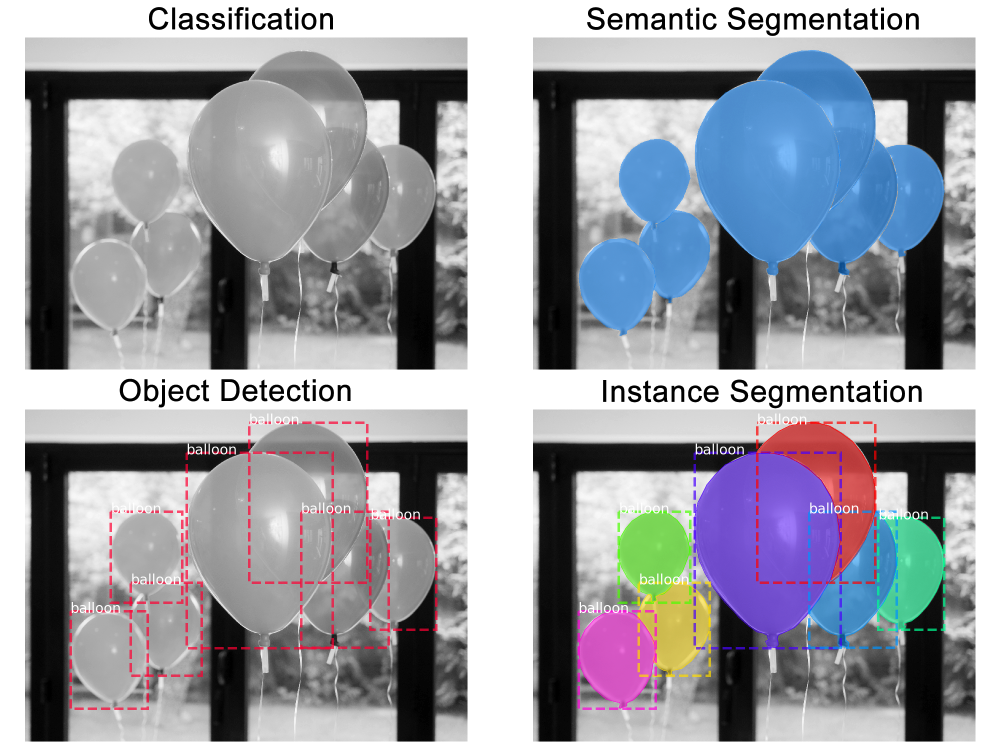
\includegraphics[scale=0.2]{figuras/image-segmentation-types}
    \source{\cite{MediumInstanceSegmentation2019}}
  \end{figure}
\end{frame}

%% ---------------------------------------------------------------------------
\subsection{Subseção I}
\begin{frame}{Criando Blocos}
    % Blocks styles
    \begin{block}{Bloco Padrão}
        Texto do corpo do bloco.
    \end{block}

    \begin{alertblock}{Bloco de Alerta}
        Texto do corpo do bloco.
    \end{alertblock}

    \begin{exampleblock}{Bloco de Exemplo}
        Texto do corpo do bloco.
    \end{exampleblock}
\end{frame}

%% ---------------------------------------------------------------------------
\subsection{Subseção II}
\begin{frame}{Criando Caixas}
    \successbox{testando o success box}

    \pause

    \alertbox{testando o alert box}

    \pause

    \simplebox{testando o simple box}
\end{frame}

% This frame show an example to insert multicolumns
\section{Multicolunas}
\begin{frame}{Seção II - Multicolunas}
    \begin{columns}{}
        \begin{column}{0.5\textwidth}
            \justify
            É possível colocar mais de uma coluna utilizando os comandos de $\backslash$begin\{column\}\{\} e $\backslash$end\{column\}
        \end{column}
        \begin{column}{0.5\textwidth}
            \justify
            Porém, o espaçamento deve ser proporcional entre as colunas para que estas colunas não entrem em coflito. O espaçamento é dado pelo segundo argumento do $\backslash$begin.
        \end{column}
    \end{columns}
\end{frame}

%% ---------------------------------------------------------------------------
% This frame show an example to insert figures
\section{Imagens}
\begin{frame}{Seção III - Figures}
    \begin{figure}
        \centering
        \caption{Emblema da UFC.}
        \includegraphics[scale=0.3]{templatebeamerufc/libs/emblemufc.pdf}
        \source{Obtido pelo site oficial da UFC ...}
        \label{fig:ufc_emblem}
    \end{figure}
\end{frame}

%% ---------------------------------------------------------------------------
% Reference frames
\begin{frame}[allowframebreaks]
    \frametitle{Referências}
    \printbibliography{}
\end{frame}

%% ---------------------------------------------------------------------------
% Final frame
\begin{frame}{}
    \centering
    \huge{\textbf{\example{Obrigado pela atenção!}}}

    \vspace{1cm}

    \Large{\textbf{Contato:}}
    \newline
    \vspace*{0.5cm}
    \large{\email{manoel.machado@alu.ufc.br}}
\end{frame}

\end{document}
